\section{Spezialthemen}


\subsection{XXE File Inclusion}
Unter dem Begriff ist eine Attacke über das \textit{XML External Entity Processing} möglich. Dabei können externe Daten, wie z.B. lokale Dateien, in das XML inkludiert werden. Bei der Verarbeitung solcher Inclusions, welche im DTD angegeben sind, fügt sie der Parser in die angegebenen Stelle ein.\\

\textbf{Lösung:} Deaktivierung des Features für DTDs (External Entities) beim Parser.

\begin{lstlisting}[language=XML, caption=Beispiel der XXE]
<?xml version="1.0" encoding="ISO-8859-1"?>
<!DOCTYPE foo [  
  <!ELEMENT foo ANY >
  <!ENTITY xxe SYSTEM "file:///etc/passwd" >]>
<foo>&xxe;</foo>
\end{lstlisting}

\subsection{JSON-Hijacking}
JSON-Hijacking zielt darauf ab, sensitive Daten, die mittels JSON Format an einen authentifizierten Empfänger übermittelt werden, zu stehlen. Dabei präpariert der Angreifer eine Seite mit einem JavaScript, welches die Callback-Funktion oder den \textit{Property Setter} überschreibt. Als zweites wird ein GET Request auf die verwundbare Seite durchgeführt. Die Response kann dann vom Angreifer verarbeitet werden und die Daten (möglicherweise sensitive Informationen) auf seinem System speichern.\\

\textbf{Lösung:}
\begin{easylist}
	& Token in Request URLs verwenden, sodass diese nicht erraten werden können
	& JSON Response mit einem Infinite Loop beginnen
	& JSONP vermeiden
	& Arrays in ein JSON-Objekt einbetten
\end{easylist} 

\subsection{URL-Redirection}
URL-Redirection wird häufig im Zusammenhang mit Phishing verwendet, mit dem Ziel, eine Session übernehmen zu können. Dazu wird dem Opfer einen Link untergeschoben, der auf den ersten Blick vertrauenswürdig aussieht. In Wirklichkeit enthält dieser jedoch einen Redirect auf eine Landing-Page des Hackers. Klickt das Opfer auf diesen Link, so wird normal das Login-Formular der vertrauenswürdigen Webseite geladen. Gibt das Opfer nun seine Credentials ein, werden diese auf Korrektheit geprüft und es wird eine Session ausgestellt. Nach dem erfolgreichen Login, wird nun durch Redirection nicht die vertrauenswürdige Webseite geladen, sondern die Landing-Page des Hackers. Dadurch sieht der Hacker im Log seiner Page die ausgestellte Session und kann diese übernehmen. Das Opfer selbst erhält nur eine Meldung, dass die gewünschte Seite nicht erreichbar ist. \\

\textbf{Beispiel:} http://www.example.com/login?redirect=http://www.hack.er \\

\textbf{Lösung:}
\begin{easylist}
	& Inputvalidierung
	&& Parameter die Redirect URLS enthalten validieren
	&& Prüfen ob URL wirklich zur Seite gehört
	& Lookup Tables
	&& Erstellen von Mappings zwischen Parameter und URL
	&& redirect=1
	&& redirect=acc
\end{easylist} 

\subsection{HTTP Request Smuggling}
HTTP Request Smuggling Attacken werden benutzt, um beispielsweise WAFs zu umgehen. Dabei wird die Schwachstelle ausgenutzt, dass verschiedene Sicherheitssysteme HTTP Requests unterschiedlich interpretieren. Beispielsweise kann mit CR/LF (Carriage Return / Line Feed) erreicht werden, dass innerhalb eines einzigen Requests sich zwei Requests befinden. Die WAF erkennt nur den einen, der dahinter verborgene Webserver antwortet jedoch auf beide Requests. Somit können Informationen, die eigentlich nur zwischen WAF und Webserver sichtbar sein sollten, nach "'aussen"' gelangen. Beispielsweise ein Cookie welches zwischen WAF und Webserver einen User authentifiziert.\\

Oftmals werden die Felder Location und Set-Cookie als Ziel verwendet. Übliche Escape-Sequenzen sind: \lstinline|%0a %0d %0a%0d %0d%0a|

\begin{lstlisting}[language={},caption=Beispiel eines Präparierten Request zur Umgehung einer Pre-Authentication]
username=hacker10&url=%2Fsecure%0aSet-Cookie:LOGON=OK; %0aSet-Cookie:MOD_BUT_Username=admin;&lang=EN&password=compass
\end{lstlisting}

\textbf{Lösung:}
\begin{easylist}
	& Web Application Firewalls verwenden, die nicht verwundbar gegen HTTP Request Smuggling sind.
	& Strenges Sessionmanagement verwenden, z.B Session nach jedem Request terminieren.
	& Aktivieren von Strict Parsing beim Webserver, z.B. Apache.
\end{easylist} 

\subsection{Session Fixation}
Bei einer Session Fixation Attacke erzeugt der Hacker bei der verwundbaren Webseite eine Session (ohne Login). Diese Session wird nun dem Opfer mit einem Link mitgeteilt. Das Opfer authentifiziert sich auf der Webseite unter Verwendung dieser Session und ermöglicht es somit dem Hacker, die authentifizierte Session zu benützen.

\subsection{SSL/TLS: SSL-Cipher-Suite-Hardening, SSL-MitM}

\subsubsection{Apache SSL Cipher Hardening}
Der Nachteil des Apache SSL Cipher Hardening ist, dass der Benutzer eine unfreundliche Error-Nachricht erhält, falls dieser den Angeforderten SSL Cipher nicht unterstützt.
\begin{easylist}
	& SSLProtocol
	&& Definiert, welche protokolle akzeptiert werden
	& SSL-Cipher-Suite-Hardening
	&& Definiert, welche SSL-Cipher akzeptiert wird
	& SSLHonorCipherOrder
	&& Die Server SSL-Cipher Suit hat mehr priorität als die des Clients.
\end{easylist}
\begin{figure}[H]
	\centering
	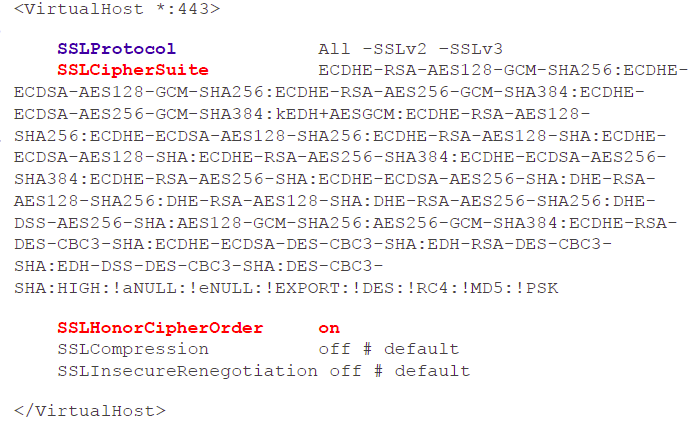
\includegraphics[width=0.8\textwidth]{./img/apache_ssl_configuration.png}
	\caption{Apache SSL Configuraiton}
\end{figure}

\subsubsection{Apache SSL Cipher Forwarding}
Der Vorteil dieser Variante ist, dass auch ältere Browsers sich mit der Applikation verbinden können, da der Apache alle Ciphers akzeptiert.\\

Apache leitet dann die SSL Informationen zu der Applikation,  via dem mod\_header weiter, welche dann den Entscheid für die entsprechende SSL Cipher Suit macht.
\begin{easylist}
	& Applikation muss die Cipher prüfen
	& Bei Änderungen oder neuen Cipher muss die Applikation neu konfiguriert werden.
\end{easylist}	
